\documentclass[12pt]{article}
\usepackage{amsmath}
\usepackage{graphicx,psfrag,epsf}
\usepackage{enumerate}
\usepackage{natbib}
\usepackage{tcolorbox}
\usepackage{url} % not crucial - just used below for the URL
\providecommand{\tightlist}{%
  \setlength{\itemsep}{0pt}\setlength{\parskip}{0pt}}

%\pdfminorversion=4
% NOTE: To produce blinded version, replace "0" with "1" below.
\newcommand{\blind}{0}

% need this for pandoc %
\newlength{\cslhangindent}
\setlength{\cslhangindent}{1.5em}
\newlength{\csllabelwidth}
\setlength{\csllabelwidth}{3em}
\newenvironment{CSLReferences}[3] % #1 hanging-ident, #2 entry spacing
 {% don't indent paragraphs
  \setlength{\parindent}{0pt}
  % turn on hanging indent if param 1 is 1
  \ifodd #1 \everypar{\setlength{\hangindent}{\cslhangindent}}\ignorespaces\fi
  % set entry spacing
  \ifnum #2 > 0
  \setlength{\parskip}{#2\baselineskip}
  \fi
 }%
 {}
\usepackage{calc} % for \widthof, \maxof
\newcommand{\CSLBlock}[1]{#1\hfill\break}
\newcommand{\CSLLeftMargin}[1]{\parbox[t]{\maxof{\widthof{#1}}{\csllabelwidth}}{#1}}
\newcommand{\CSLRightInline}[1]{\parbox[t]{\linewidth}{#1}}
\newcommand{\CSLIndent}[1]{\hspace{\cslhangindent}#1}


% DON'T change margins - should be 1 inch all around.
\addtolength{\oddsidemargin}{-.5in}%
\addtolength{\evensidemargin}{-.5in}%
\addtolength{\textwidth}{1in}%
\addtolength{\textheight}{1.3in}%
\addtolength{\topmargin}{-.8in}%

%-------------------------------------------------------------------
% R MARKDOWN
%-------------------------------------------------------------------
\IfFileExists{bookmark.sty}{\usepackage{bookmark}}{\usepackage{hyperref}}

\def\spacingset#1{\renewcommand{\baselinestretch}%
{#1}\small\normalsize} \spacingset{1}

\usepackage{color}
\usepackage{fancyvrb}
\newcommand{\VerbBar}{|}
\newcommand{\VERB}{\Verb[commandchars=\\\{\}]}
\DefineVerbatimEnvironment{Highlighting}{Verbatim}{commandchars=\\\{\}}
% Add ',fontsize=\small' for more characters per line
\usepackage{framed}
\definecolor{shadecolor}{RGB}{248,248,248}
\newenvironment{Shaded}{\begin{snugshade}}{\end{snugshade}}
\newcommand{\AlertTok}[1]{\textcolor[rgb]{0.94,0.16,0.16}{#1}}
\newcommand{\AnnotationTok}[1]{\textcolor[rgb]{0.56,0.35,0.01}{\textbf{\textit{#1}}}}
\newcommand{\AttributeTok}[1]{\textcolor[rgb]{0.77,0.63,0.00}{#1}}
\newcommand{\BaseNTok}[1]{\textcolor[rgb]{0.00,0.00,0.81}{#1}}
\newcommand{\BuiltInTok}[1]{#1}
\newcommand{\CharTok}[1]{\textcolor[rgb]{0.31,0.60,0.02}{#1}}
\newcommand{\CommentTok}[1]{\textcolor[rgb]{0.56,0.35,0.01}{\textit{#1}}}
\newcommand{\CommentVarTok}[1]{\textcolor[rgb]{0.56,0.35,0.01}{\textbf{\textit{#1}}}}
\newcommand{\ConstantTok}[1]{\textcolor[rgb]{0.00,0.00,0.00}{#1}}
\newcommand{\ControlFlowTok}[1]{\textcolor[rgb]{0.13,0.29,0.53}{\textbf{#1}}}
\newcommand{\DataTypeTok}[1]{\textcolor[rgb]{0.13,0.29,0.53}{#1}}
\newcommand{\DecValTok}[1]{\textcolor[rgb]{0.00,0.00,0.81}{#1}}
\newcommand{\DocumentationTok}[1]{\textcolor[rgb]{0.56,0.35,0.01}{\textbf{\textit{#1}}}}
\newcommand{\ErrorTok}[1]{\textcolor[rgb]{0.64,0.00,0.00}{\textbf{#1}}}
\newcommand{\ExtensionTok}[1]{#1}
\newcommand{\FloatTok}[1]{\textcolor[rgb]{0.00,0.00,0.81}{#1}}
\newcommand{\FunctionTok}[1]{\textcolor[rgb]{0.00,0.00,0.00}{#1}}
\newcommand{\ImportTok}[1]{#1}
\newcommand{\InformationTok}[1]{\textcolor[rgb]{0.56,0.35,0.01}{\textbf{\textit{#1}}}}
\newcommand{\KeywordTok}[1]{\textcolor[rgb]{0.13,0.29,0.53}{\textbf{#1}}}
\newcommand{\NormalTok}[1]{#1}
\newcommand{\OperatorTok}[1]{\textcolor[rgb]{0.81,0.36,0.00}{\textbf{#1}}}
\newcommand{\OtherTok}[1]{\textcolor[rgb]{0.56,0.35,0.01}{#1}}
\newcommand{\PreprocessorTok}[1]{\textcolor[rgb]{0.56,0.35,0.01}{\textit{#1}}}
\newcommand{\RegionMarkerTok}[1]{#1}
\newcommand{\SpecialCharTok}[1]{\textcolor[rgb]{0.00,0.00,0.00}{#1}}
\newcommand{\SpecialStringTok}[1]{\textcolor[rgb]{0.31,0.60,0.02}{#1}}
\newcommand{\StringTok}[1]{\textcolor[rgb]{0.31,0.60,0.02}{#1}}
\newcommand{\VariableTok}[1]{\textcolor[rgb]{0.00,0.00,0.00}{#1}}
\newcommand{\VerbatimStringTok}[1]{\textcolor[rgb]{0.31,0.60,0.02}{#1}}
\newcommand{\WarningTok}[1]{\textcolor[rgb]{0.56,0.35,0.01}{\textbf{\textit{#1}}}}

\begin{document}

%\bibliographystyle{natbib}

\def\spacingset#1{\renewcommand{\baselinestretch}%
{#1}\small\normalsize} \spacingset{1}


%%%%%%%%%%%%%%%%%%%%%%%%%%%%%%%%%%%%%%%%%%%%%%%%%%%%%%%%%%%%%%%%%%%%%%%%%%%%%%

\if0\blind
{
  \title{\bf The Journey from Wild to Textbook Data: A Case Study from the National Longitudinal Survey of Youth}
  \author{
            Dewi Amaliah\thanks{Test}\\
      Department of Econometrics and Business Statistics, Monash University, \\
            Dianne Cook\\
      Department of Econometrics and Business Statistics, Monash University, \\
            Emi Tanaka\\
      Department of Econometrics and Business Statistics, Monash University, \\
            Kate Hyde\\
      Department of Econometrics and Business Statistics, Monash University, \\
            Nicholas Tierney\\
      , , }
        \maketitle
} \fi

\if1\blind
{
  \bigskip
  \bigskip
  \bigskip
  \begin{center}
    {\LARGE\bf Title}
\end{center}
  \medskip
} \fi

\bigskip
\begin{abstract}

\end{abstract}

\noindent%
{\it Keywords:}  3 to 6 keywords, that do not appear in the title
\vfill

\newpage
\spacingset{1.45} % DON'T change the spacing!

\textbf{Keywords}: Data cleaning; Data tidying; Longitudinal data; NLSY79; Open data; Initial data analysis; Outlier detection; Robust linear regression

\hypertarget{intro}{%
\section{Introduction}\label{intro}}

``Open data'' is data that is freely accessible, modifiable, and shareable by anyone for any purpose (Open Knowledge Foundation 2021). This type of data can be useful as example data in statistical textbooks and for research purposes. However, open data is often referred to as what we might call ``wild data'' because it requires substantial cleaning and tidying to tame it into textbook shape. Huebner Marianne, Vach, and Cessie (2016) emphasize that making the data cleaning process accountable and transparent is imperative. Documenting the data cleaning is essential for the integrity of downstream statistical analyses and model building (M. Huebner et al. 2020).
Data cleaning can be considered to be a part of what is called ``initial data analysis (IDA)'' (Chatfield 1985). In IDA one would also explore the data, especially to check if the dta is consistent with assumptions required for modeling. This is also related to exploratory data analysis, which Tukey (1977) defines as detective work to learn from data, either numerically or graphically, before confirmatory data analysis is performed, encompasses IDA. Dasu and Johnson (2003) say that data cleaning and exploration, without naming it as IDA, is a difficult task and consumes 80\% of the data mining task.

Despite its importance, this IDA stage is often undervalued and neglected (Chatfield 1985). There are few research papers that document the data cleaning (Wickham 2014). Furthermore, the decisions made in this stage often go unreported in the sense that IDA is often performed in an unplanned and unstructured way and is only shared among restricted parties (M. Huebner et al. 2020).

This paper aims to demonstrate the steps of IDA, tidying, cleaning, and documenting the process, for a prominent open data source, National Longitudinal Survey of Youth (NLSY) 1979, henceforth referred to NLSY79. This data has been playing an important role in research in various disciplines, including but are not limited to economics, sociology, education, public policy, and public health for more than a quarter of the century (Pergamit et al. 2001). In addition, The National Longitudinal Survey is considered a survey with high retention rates and carefully designed, making it suitable for a life course research (Pergamit et al. 2001) and (Cooksey 2017). According to Cooksey (2017), thousand of articles, and hundreds of book chapters and monographs has incorporated the NLSY data. Moreover, the NLSY79 is considered the most widely used and most important cohort in the NLSY79 data sets (Pergamit et al. 2001).

Singer and Willett (2003) used the wages and other variables of high school dropouts from the NLSY79 data as an example data set to illustrate longitudinal data modeling. Our aim is to refresh this textbook data to be more up to date. Here, we investigate the process of getting from the raw NLSY79 to this textbook data set. However, we cannot create the exact same data set as published in their book since we do not have the information of what age threshold they used to determine the high school dropouts.

This paper is structured to have 5 sections. Section \ref{database} describes the original data source. Section \ref{cleaning} presents the steps of cleaning the data, including getting and tidying the data from the NLSY79 and initial data analysis to find and treat the anomalies in the data. We also gave examples of exploratory data analysis using the clean data in Section \ref{eda}. Finally, Section \ref{summary} summarises the paper.

\hypertarget{database}{%
\section{The NLSY79}\label{database}}

\hypertarget{database-1}{%
\subsection{Database}\label{database-1}}

The NLSY79 is a longitudinal survey held by the U.S Bureau of Labor Statistics that follows the lives of a sample of American youth and born between 1957-1964 (The U.S. Bureau of Labor Statistics, n.d.). The cohort originally included 12,686 respondents ages 14-22 when first interviewed in 1979. It was comprised of Blacks, Hispanics, economically disadvantaged non-Black non-Hispanics, and youth in the military. In 1984 and 1990, two sub-samples were dropped from the interview; the dropped subjects are the 1,079 members of the military sample and 1,643 members of the economically disadvantaged non-Black non-Hispanics, respectively. Hence, 9,964 respondents remain in the eligible samples. The surveys were conducted annually from 1979 to 1994 and biennially thereafter. Data are now available from Round 1 (1979 survey year) to Round 28 (2018 survey year).

{[}FILL{]} We should include how many variables there are in the data so people get a grasp of the extensive coverage of the variables.

Although the main focus area of the NLSY is labor and employment, the NLSY also covers several other topics, including education; training and achievement; household, geography, and contextual variables; dating, marriage, cohabitation; sexual activity, pregnancy, and fertility; children; income, assets and program participation; health; attitudes and expectations; and crime and substance use.

There are two ways to conduct the interview of the NLSY79, which are face-to-face interviews or by telephone. In recent survey years, more than 90 percent of respondents were interviewed by telephone (Cooksey 2017).

\hypertarget{target-data}{%
\subsection{Target Data}\label{target-data}}

As mentioned in Section \ref{intro}, this paper aims to refresh the NLSY79 data as used in Singer and Willet's textbook (Singer and Willett (2003)). This data set contains the information of yearly mean hourly wages from the NLSY79 cohort, with education and race as covariates. This data set represents the measurement of male high-school dropouts, aged from 14 to 17 years old when first time measured. Accordingly, to get this data, we have two additional target data, NLSY79 cohort's demographic profiles and wages data of people who completed education up to high school.

Since there is no information on high school dropouts in Singer and Willet's book, we define high school dropouts as respondents who only completed either \(9^{th}\), \(10^{th}\), \(11^{th}\) grade, or who completed \(12^{th}\) when their age is at least 19 years old (means that these IDs being dropped out in a certain year, but they returned back to high school to complete it).

\hypertarget{cleaning}{%
\section{Data Cleaning}\label{cleaning}}

\hypertarget{getting-and-tidying-the-data}{%
\subsection{Getting and Tidying the Data}\label{getting-and-tidying-the-data}}

The NLSY79 data are stored in a \href{https://www.nlsinfo.org/content/cohorts/nlsy79/get-data}{database} and could be downloaded by variables. Several variables are available for download and could be browsed by index. For the wages data set, we only extracted these variables:

\begin{tcolorbox}[width=\textwidth,
                  boxsep=5pt,
                  left=5pt,
                  right=5pt,
                  top=5pt,
                  ]
Education, Training and Achievement Scores

- Education -> Summary measures -> All schools -> By year -> Highest grade completed
  - Downloaded all of variables in Highest grade completed.
  
Employment

- Summary measures -> By job -> Hours worked and Hourly wages
  - Downloaded all of the variables in Hours worked.
  - Downloaded all of the variables in Hourly wages
  Both hours worked and hourly wages are recorded by the job, up to five jobs for each id/subject. 
  
Household, Geography and Contextual Variables

- Context -> Summary measures -> Basic demographics 
  - Downloaded year and month of birth, race, and sex variables.
  There are two versions of the year and month of birth, i.e., 1979 and 1981 data. We downloaded these two versions.

\end{tcolorbox}

The downloaded data set came in a csv (NLSY79.csv) and dat (NLSY79.dat) format. We only used the .dat format. It also came along with these files:

\begin{itemize}
\tightlist
\item
  NLSY79.NLSY79: Tagset of variables that can be uploaded to the website to recreate the data set.
\item
  NLSY79.R: R script provided automatically by the database for reading the data into R and converting the variables' names and label into something more sensible. We utilized this code to do an initial data tidying. It produced two data set, \texttt{categories\_qnames} (the observations are stored in categorical/interval values) and \texttt{new\_data\_qnames} (the observations are stored in integer form).
\end{itemize}

According to Wickham (2014), tidy data sets comply with three rules. Firstly, each variable forms a column. Secondly, each observation forms a row. Lastly, each type of observational unit forms a table. Unfortunately, the \texttt{new\_data\_qnames} did not meet these requirements in the way that data for each year and job for the same respondent is stored as one variable. Hence, the data contains a huge number of columns (686 columns). The example of the untidy data set is displayed in Table \ref{tab:untidy-data}. The table intended to display the hourly rate of each respondent by job (HRP1 to HRP5) and by year (1979 and 1980). The table implies that the column headers are values of the year and job, not variable names. Consequently, the data should be tidied and wrangled first to extract the demographic and employment variables we want to put in the final data set. We mainly used \texttt{tidyr} (Wickham 2020b), \texttt{dplyr} (Wickham et al. 2020), and \texttt{stringr} (Wickham 2019) to do this job.

\begin{table}

\caption{\label{tab:untidy-data}The Untidy Form of the NLSY79 Raw Data}
\centering
\begin{tabular}[t]{r|r|r|r|r|r|r}
\hline
CASEID\_1979 & HRP1\_1979 & HRP2\_1979 & HRP3\_1979 & HRP4\_1979 & HRP5\_1979 & HRP1\_1980\\
\hline
1 & 328 & NA & NA & NA & NA & NA\\
\hline
2 & 385 & NA & NA & NA & NA & 457\\
\hline
3 & 365 & NA & 275 & NA & NA & 397\\
\hline
4 & NA & NA & NA & NA & NA & NA\\
\hline
5 & 310 & 375 & NA & NA & NA & 333\\
\hline
6 & NA & NA & NA & 250 & NA & 275\\
\hline
\end{tabular}
\end{table}

\hypertarget{tidying-demographic-variables}{%
\subsubsection{Tidying demographic variables}\label{tidying-demographic-variables}}

\texttt{Age\ in\ 1979}, \texttt{gender}, \texttt{race}, \texttt{highest\ grade\ completed}, and the \texttt{year\ when\ the\ highest\ grade\ completed} are the variables that we want to use in the cleaned data set.

Age in 1979 are derived from year and month of birth variables in the raw data. The variables have two versions, which are the 1979 version and the 1981 version. We only used the 1979 data and did a consistency check of those years and flag the inconsistent observations.

\begin{Shaded}
\begin{Highlighting}[]
\CommentTok{\#tidy the date of birth data}
\NormalTok{dob\_tidy }\OtherTok{\textless{}{-}}\NormalTok{ new\_data\_qnames }\SpecialCharTok{\%\textgreater{}\%}
\NormalTok{  dplyr}\SpecialCharTok{::}\FunctionTok{select}\NormalTok{(CASEID\_1979,}
                \FunctionTok{starts\_with}\NormalTok{(}\StringTok{"Q1{-}3\_A\textasciitilde{}"}\NormalTok{)) }\SpecialCharTok{\%\textgreater{}\%}
  \FunctionTok{mutate}\NormalTok{(}\AttributeTok{dob\_year =} \FunctionTok{case\_when}\NormalTok{(}
    \CommentTok{\# if the years recorded in both sets match, take 79 data}
    \StringTok{\textasciigrave{}}\AttributeTok{Q1{-}3\_A\textasciitilde{}Y\_1979}\StringTok{\textasciigrave{}} \SpecialCharTok{==} \StringTok{\textasciigrave{}}\AttributeTok{Q1{-}3\_A\textasciitilde{}Y\_1981}\StringTok{\textasciigrave{}} \SpecialCharTok{\textasciitilde{}} \StringTok{\textasciigrave{}}\AttributeTok{Q1{-}3\_A\textasciitilde{}Y\_1979}\StringTok{\textasciigrave{}}\NormalTok{,}
    \CommentTok{\# if the year in the 81 set is missing, take the 79 data}
    \FunctionTok{is.na}\NormalTok{(}\StringTok{\textasciigrave{}}\AttributeTok{Q1{-}3\_A\textasciitilde{}Y\_1981}\StringTok{\textasciigrave{}}\NormalTok{) }\SpecialCharTok{\textasciitilde{}} \StringTok{\textasciigrave{}}\AttributeTok{Q1{-}3\_A\textasciitilde{}Y\_1979}\StringTok{\textasciigrave{}}\NormalTok{,}
    \CommentTok{\# if the sets don\textquotesingle{}t match for dob year, take the 79 data}
    \StringTok{\textasciigrave{}}\AttributeTok{Q1{-}3\_A\textasciitilde{}Y\_1979}\StringTok{\textasciigrave{}} \SpecialCharTok{!=} \StringTok{\textasciigrave{}}\AttributeTok{Q1{-}3\_A\textasciitilde{}Y\_1981}\StringTok{\textasciigrave{}} \SpecialCharTok{\textasciitilde{}} \StringTok{\textasciigrave{}}\AttributeTok{Q1{-}3\_A\textasciitilde{}Y\_1979}\StringTok{\textasciigrave{}}\NormalTok{),}
    \AttributeTok{dob\_month =} \FunctionTok{case\_when}\NormalTok{(}
      \CommentTok{\# if months recorded in both sets match, take 79 data}
      \StringTok{\textasciigrave{}}\AttributeTok{Q1{-}3\_A\textasciitilde{}M\_1979}\StringTok{\textasciigrave{}} \SpecialCharTok{==} \StringTok{\textasciigrave{}}\AttributeTok{Q1{-}3\_A\textasciitilde{}M\_1981}\StringTok{\textasciigrave{}} \SpecialCharTok{\textasciitilde{}} \StringTok{\textasciigrave{}}\AttributeTok{Q1{-}3\_A\textasciitilde{}M\_1979}\StringTok{\textasciigrave{}}\NormalTok{,}
      \CommentTok{\# if month in 81 set is missing, take the 79 data}
      \FunctionTok{is.na}\NormalTok{(}\StringTok{\textasciigrave{}}\AttributeTok{Q1{-}3\_A\textasciitilde{}M\_1981}\StringTok{\textasciigrave{}}\NormalTok{) }\SpecialCharTok{\textasciitilde{}} \StringTok{\textasciigrave{}}\AttributeTok{Q1{-}3\_A\textasciitilde{}M\_1979}\StringTok{\textasciigrave{}}\NormalTok{,}
      \CommentTok{\# if sets don\textquotesingle{}t match for dob month, take the 79 data}
      \StringTok{\textasciigrave{}}\AttributeTok{Q1{-}3\_A\textasciitilde{}M\_1979}\StringTok{\textasciigrave{}} \SpecialCharTok{!=} \StringTok{\textasciigrave{}}\AttributeTok{Q1{-}3\_A\textasciitilde{}M\_1981}\StringTok{\textasciigrave{}} \SpecialCharTok{\textasciitilde{}} \StringTok{\textasciigrave{}}\AttributeTok{Q1{-}3\_A\textasciitilde{}M\_1979}\StringTok{\textasciigrave{}}\NormalTok{),}
    \CommentTok{\# flag if there is a conflict between dob recorded in 79 and 81}
    \AttributeTok{dob\_conflict =} \FunctionTok{case\_when}\NormalTok{(}
\NormalTok{      (}\StringTok{\textasciigrave{}}\AttributeTok{Q1{-}3\_A\textasciitilde{}M\_1979}\StringTok{\textasciigrave{}} \SpecialCharTok{!=} \StringTok{\textasciigrave{}}\AttributeTok{Q1{-}3\_A\textasciitilde{}M\_1981}\StringTok{\textasciigrave{}}\NormalTok{) }\SpecialCharTok{\&} \SpecialCharTok{!}\FunctionTok{is.na}\NormalTok{(}\StringTok{\textasciigrave{}}\AttributeTok{Q1{-}3\_A\textasciitilde{}M\_1981}\StringTok{\textasciigrave{}}\NormalTok{)}
      \SpecialCharTok{\textasciitilde{}} \ConstantTok{TRUE}\NormalTok{,}
\NormalTok{      (}\StringTok{\textasciigrave{}}\AttributeTok{Q1{-}3\_A\textasciitilde{}Y\_1979}\StringTok{\textasciigrave{}} \SpecialCharTok{!=} \StringTok{\textasciigrave{}}\AttributeTok{Q1{-}3\_A\textasciitilde{}Y\_1981}\StringTok{\textasciigrave{}}\NormalTok{) }\SpecialCharTok{\&} \SpecialCharTok{!}\FunctionTok{is.na}\NormalTok{(}\StringTok{\textasciigrave{}}\AttributeTok{Q1{-}3\_A\textasciitilde{}Y\_1981}\StringTok{\textasciigrave{}}\NormalTok{)}
      \SpecialCharTok{\textasciitilde{}} \ConstantTok{TRUE}\NormalTok{,}
\NormalTok{      (}\StringTok{\textasciigrave{}}\AttributeTok{Q1{-}3\_A\textasciitilde{}Y\_1979}\StringTok{\textasciigrave{}} \SpecialCharTok{==} \StringTok{\textasciigrave{}}\AttributeTok{Q1{-}3\_A\textasciitilde{}Y\_1981}\StringTok{\textasciigrave{}}\NormalTok{) }\SpecialCharTok{\&}
\NormalTok{        (}\StringTok{\textasciigrave{}}\AttributeTok{Q1{-}3\_A\textasciitilde{}M\_1979}\StringTok{\textasciigrave{}} \SpecialCharTok{==} \StringTok{\textasciigrave{}}\AttributeTok{Q1{-}3\_A\textasciitilde{}M\_1981}\StringTok{\textasciigrave{}}\NormalTok{) }\SpecialCharTok{\textasciitilde{}} \ConstantTok{FALSE}\NormalTok{,}
      \FunctionTok{is.na}\NormalTok{(}\StringTok{\textasciigrave{}}\AttributeTok{Q1{-}3\_A\textasciitilde{}M\_1981}\StringTok{\textasciigrave{}}\NormalTok{) }\SpecialCharTok{|} \FunctionTok{is.na}\NormalTok{(}\StringTok{\textasciigrave{}}\AttributeTok{Q1{-}3\_A\textasciitilde{}Y\_1981}\StringTok{\textasciigrave{}}\NormalTok{) }\SpecialCharTok{\textasciitilde{}} \ConstantTok{FALSE}\NormalTok{)) }\SpecialCharTok{\%\textgreater{}\%}
\NormalTok{  dplyr}\SpecialCharTok{::}\FunctionTok{select}\NormalTok{(CASEID\_1979,}
\NormalTok{                dob\_month,}
\NormalTok{                dob\_year,}
\NormalTok{                dob\_conflict)}
\end{Highlighting}
\end{Shaded}

For \texttt{gender} and \texttt{race}, we only rename the column names. It is worth noting that using these two variable needs special attention. Gender, as reported in the data, only has two categories, which is recognised today as inadequate. Gender is not binary. Further, race is as reported in the database. When doing analysis with this variable, one should keep in mind that the purpose is to study racism rather than race.

The next step is tidying the \texttt{highest\ grade\ completed} variable. This variable came with several version in each year. We choose the revised May data because it seemed to have less missing and presumably has been checked. However, there is no revised May data for 2012, 2014, 2016, and 2018. Thus, we just use the ordinary May data for these years. The code for tidying this variable is provided in the supplementary materials.

Further, \texttt{highest\ grade\ completed} is measured and could be updated in each period of the survey. Hence, we only used the highest grade completed ever and derived the year when it is completed. The code for tidying this variable is also available in the supplementary materials.

Finally, we get all of the demographic profiles of the NLSY79 cohort. We then save this data as \texttt{demog\_nlsy79}.

\hypertarget{tidying-employment-variables}{%
\subsubsection{Tidying employment variables}\label{tidying-employment-variables}}

The employment data comprises of three variables, i.e., \texttt{total\ hours\ of\ work\ per\ week}, \texttt{number\ of\ jobs\ that\ an\ individual\ has}, and \texttt{mean\ hourly\ wage}.

\texttt{hours\ worked\ per\ week} initially has only one version per job, no choice from 1979 to 1987 (QES-52A). From 1988 onward, when we had more options, we chose the variable for total hours, including time spent working from home (QES-52D). However, in 1993, this variable did not have all the five D variables (the first one and the last one were missing), so we used QES-52A variable instead. In addition, 2008 only had jobs 1-4 for the QES-52D variable (whereas the other years had 1-5), so we use these.

\begin{Shaded}
\begin{Highlighting}[]
\CommentTok{\# make a list for years where we used the "QES{-}52A"}
\NormalTok{year\_A }\OtherTok{\textless{}{-}} \FunctionTok{c}\NormalTok{(}\DecValTok{1979}\SpecialCharTok{:}\DecValTok{1987}\NormalTok{, }\DecValTok{1993}\NormalTok{)}
\CommentTok{\#function to get the hour of work}
\NormalTok{get\_hour }\OtherTok{\textless{}{-}} \ControlFlowTok{function}\NormalTok{(year)\{}
  \ControlFlowTok{if}\NormalTok{(year }\SpecialCharTok{\%in\%}\NormalTok{ year\_A)\{}
\NormalTok{    temp }\OtherTok{\textless{}{-}}\NormalTok{ new\_data\_qnames }\SpecialCharTok{\%\textgreater{}\%}
\NormalTok{      dplyr}\SpecialCharTok{::}\FunctionTok{select}\NormalTok{(CASEID\_1979,}
                    \FunctionTok{starts\_with}\NormalTok{(}\StringTok{"QES{-}52A"}\NormalTok{) }\SpecialCharTok{\&}
                      \FunctionTok{ends\_with}\NormalTok{(}\FunctionTok{as.character}\NormalTok{(year)))\}}
  \ControlFlowTok{else}\NormalTok{\{}
\NormalTok{    temp }\OtherTok{\textless{}{-}}\NormalTok{ new\_data\_qnames }\SpecialCharTok{\%\textgreater{}\%}
\NormalTok{      dplyr}\SpecialCharTok{::}\FunctionTok{select}\NormalTok{(CASEID\_1979,}
                    \FunctionTok{starts\_with}\NormalTok{(}\StringTok{"QES{-}52D"}\NormalTok{) }\SpecialCharTok{\&}
                      \FunctionTok{ends\_with}\NormalTok{(}\FunctionTok{as.character}\NormalTok{(year)))\}}
\NormalTok{  temp }\SpecialCharTok{\%\textgreater{}\%}
    \FunctionTok{pivot\_longer}\NormalTok{(}\SpecialCharTok{!}\NormalTok{CASEID\_1979,}
                 \AttributeTok{names\_to =} \StringTok{"job"}\NormalTok{,}
                 \AttributeTok{values\_to =} \StringTok{"hours\_work"}\NormalTok{) }\SpecialCharTok{\%\textgreater{}\%}
    \FunctionTok{separate}\NormalTok{(}\StringTok{"job"}\NormalTok{, }\FunctionTok{c}\NormalTok{(}\StringTok{"job"}\NormalTok{, }\StringTok{"year"}\NormalTok{), }\AttributeTok{sep =} \SpecialCharTok{{-}}\DecValTok{4}\NormalTok{) }\SpecialCharTok{\%\textgreater{}\%}
    \FunctionTok{mutate}\NormalTok{(}\AttributeTok{job =} \FunctionTok{paste0}\NormalTok{(}\StringTok{"job\_"}\NormalTok{, }\FunctionTok{substr}\NormalTok{(job, }\DecValTok{9}\NormalTok{, }\DecValTok{10}\NormalTok{))) }\SpecialCharTok{\%\textgreater{}\%}
    \FunctionTok{rename}\NormalTok{(}\AttributeTok{id =}\NormalTok{ CASEID\_1979)}
\NormalTok{\}}
\CommentTok{\# list to save the iteration result}
\NormalTok{hours }\OtherTok{\textless{}{-}} \FunctionTok{list}\NormalTok{()}
\CommentTok{\# getting the hours of work of all observations}
\ControlFlowTok{for}\NormalTok{(ayear }\ControlFlowTok{in} \FunctionTok{c}\NormalTok{(}\DecValTok{1979}\SpecialCharTok{:}\DecValTok{1994}\NormalTok{, }\DecValTok{1996}\NormalTok{, }\DecValTok{1998}\NormalTok{, }\DecValTok{2000}\NormalTok{, }\DecValTok{2002}\NormalTok{, }\DecValTok{2004}\NormalTok{, }\DecValTok{2006}\NormalTok{, }\DecValTok{2008}\NormalTok{, }\DecValTok{2010}\NormalTok{,}
               \DecValTok{2012}\NormalTok{, }\DecValTok{2014}\NormalTok{, }\DecValTok{2016}\NormalTok{, }\DecValTok{2018}\NormalTok{)) \{}
\NormalTok{  hours[[ayear]] }\OtherTok{\textless{}{-}} \FunctionTok{get\_hour}\NormalTok{(ayear)}
\NormalTok{\}}
\CommentTok{\# unlist the hours of work}
\NormalTok{hours\_all }\OtherTok{\textless{}{-}} \FunctionTok{bind\_rows}\NormalTok{(}\SpecialCharTok{!!!}\NormalTok{hours)}
\end{Highlighting}
\end{Shaded}

The same way was also deployed to tidy the rate of wage by year and by ID. The difference is that the hourly rate has only one version of each year. The hours of work and the hourly rate are then joined to calculate the number of jobs that a respondent has and their mean hourly wage. Some observations have 0 in their hourly rate and work hours, which is considered an invalid value. Thus, these observations are set to be NA. Besides, there are some observations with unusual hours of work. Here, we also censored the observations with \textgreater{} 84 hours of work a week to be NA.

\begin{Shaded}
\begin{Highlighting}[]
\NormalTok{get\_rate }\OtherTok{\textless{}{-}} \ControlFlowTok{function}\NormalTok{(year) \{}
\NormalTok{  new\_data\_qnames }\SpecialCharTok{\%\textgreater{}\%}
\NormalTok{    dplyr}\SpecialCharTok{::}\FunctionTok{select}\NormalTok{(CASEID\_1979,}
                  \FunctionTok{starts\_with}\NormalTok{(}\StringTok{"HRP"}\NormalTok{) }\SpecialCharTok{\&}
                    \FunctionTok{ends\_with}\NormalTok{(}\FunctionTok{as.character}\NormalTok{(year))) }\SpecialCharTok{\%\textgreater{}\%}
    \FunctionTok{pivot\_longer}\NormalTok{(}\SpecialCharTok{!}\NormalTok{CASEID\_1979, }\AttributeTok{names\_to =} \StringTok{"job"}\NormalTok{, }\AttributeTok{values\_to =} \StringTok{"rate\_per\_hour"}\NormalTok{) }\SpecialCharTok{\%\textgreater{}\%}
    \FunctionTok{separate}\NormalTok{(}\StringTok{"job"}\NormalTok{, }\FunctionTok{c}\NormalTok{(}\StringTok{"job"}\NormalTok{, }\StringTok{"year"}\NormalTok{), }\AttributeTok{sep =} \SpecialCharTok{{-}}\DecValTok{4}\NormalTok{) }\SpecialCharTok{\%\textgreater{}\%}
    \FunctionTok{mutate}\NormalTok{(}\AttributeTok{job =} \FunctionTok{paste0}\NormalTok{(}\StringTok{"job\_0"}\NormalTok{, }\FunctionTok{substr}\NormalTok{(job, }\DecValTok{4}\NormalTok{, }\DecValTok{4}\NormalTok{))) }\SpecialCharTok{\%\textgreater{}\%}
    \FunctionTok{rename}\NormalTok{(}\AttributeTok{id =}\NormalTok{ CASEID\_1979)}
\NormalTok{\}}
\NormalTok{rates }\OtherTok{\textless{}{-}} \FunctionTok{list}\NormalTok{()}
\ControlFlowTok{for}\NormalTok{(ayear }\ControlFlowTok{in} \FunctionTok{c}\NormalTok{(}\DecValTok{1979}\SpecialCharTok{:}\DecValTok{1994}\NormalTok{, }\DecValTok{1996}\NormalTok{, }\DecValTok{1998}\NormalTok{, }\DecValTok{2000}\NormalTok{, }\DecValTok{2002}\NormalTok{, }\DecValTok{2004}\NormalTok{, }\DecValTok{2006}\NormalTok{, }\DecValTok{2008}\NormalTok{, }\DecValTok{2010}\NormalTok{,}
               \DecValTok{2012}\NormalTok{, }\DecValTok{2014}\NormalTok{, }\DecValTok{2016}\NormalTok{, }\DecValTok{2018}\NormalTok{)) \{}
\NormalTok{  rates[[ayear]] }\OtherTok{\textless{}{-}} \FunctionTok{get\_rate}\NormalTok{(ayear)}
\NormalTok{\}}
\NormalTok{rates\_all }\OtherTok{\textless{}{-}} \FunctionTok{bind\_rows}\NormalTok{(}\SpecialCharTok{!!!}\NormalTok{rates)}
\CommentTok{\# join hours and rates variable}
\NormalTok{hours\_wages }\OtherTok{\textless{}{-}} \FunctionTok{left\_join}\NormalTok{(rates\_all,}
\NormalTok{                         hours\_all,}
                         \AttributeTok{by =} \FunctionTok{c}\NormalTok{(}\StringTok{"id"}\NormalTok{, }\StringTok{"year"}\NormalTok{, }\StringTok{"job"}\NormalTok{)) }\SpecialCharTok{\%\textgreater{}\%}
  \CommentTok{\# set the 0 value in rate\_per\_hour as NA}
  \FunctionTok{mutate}\NormalTok{(}\AttributeTok{rate\_per\_hour =} \FunctionTok{ifelse}\NormalTok{(rate\_per\_hour }\SpecialCharTok{==} \DecValTok{0}\NormalTok{, }\ConstantTok{NA}\NormalTok{,}
\NormalTok{                                rate\_per\_hour),}
         \AttributeTok{hours\_work =} \FunctionTok{ifelse}\NormalTok{(hours\_work }\SpecialCharTok{==} \DecValTok{0} \SpecialCharTok{|}\NormalTok{ hours\_work }\SpecialCharTok{\textgreater{}} \DecValTok{84}\NormalTok{, }\ConstantTok{NA}\NormalTok{, hours\_work))}
\end{Highlighting}
\end{Shaded}

Since our ultimate goal is to calculate the mean hourly wage, the number of jobs is calculated based on the availability of the \texttt{rate\_per\_hour} information. For example, the number of jobs of ID 1, based on \texttt{hours\_work}, is 2. However, since the information of hourly rate of \texttt{job\_02} is not available, the number of jobs is considered as 1.

Further, we calculated the mean hourly wage for each ID in each year using a weighted mean with the hours of work as the weight. However, there is a lot of missing value in \texttt{hours\_work} variable. In that case, we only calculated the mean hourly wage based on the arithmetic/regular mean method. Hence, we created a new variable to flag whether the mean hourly wage is weighted or regular. Additionally, if an ID only had one job, we directly used their hourly wages information and flagged it as arithmetic mean.

\begin{verbatim}
#> # A tibble: 10 x 6
#>       id  year mean_hourly_wage total_hours number_of_jobs is_wm
#>    <int> <dbl>            <dbl>       <int>          <dbl> <lgl>
#>  1     1  1979             3.28          38              1 FALSE
#>  2     1  1981             3.61          NA              1 FALSE
#>  3     2  1979             3.85          35              1 FALSE
#>  4     2  1980             4.57          NA              1 FALSE
#>  5     2  1981             5.14          NA              1 FALSE
#>  6     2  1982             5.71          35              1 FALSE
#>  7     2  1983             5.71          NA              1 FALSE
#>  8     2  1984             5.14          NA              1 FALSE
#>  9     2  1985             7.71          NA              1 FALSE
#> 10     2  1986             7.69          NA              1 FALSE
\end{verbatim}

The employment and demographic variables are then joined. We also filtered the data to only have the cohort who completed the education up to 12th grade and participated at least five rounds in the survey and save it to an object called \texttt{wages}.

\hypertarget{initial-data-analysis}{%
\subsection{Initial Data Analysis}\label{initial-data-analysis}}

According to Huebner Marianne, Vach, and Cessie (2016), Initial Data Analysis (IDA) is the step of inspecting and screening the data after being collected to ensure that the data is clean, valid, and ready to be deployed in the later formal statistical analysis. Moreover, Chatfield (1985) argues that the two main objectives of IDA are data description, which is to assess the structure and the quality of the data, and model formulation without any formal statistical inference.

In this paper, we conduct an IDA or a preliminary data analysis to assess the consistency of the data with the cohort information that the NLSY provides. In addition, we also aim to find the anomaly in the wages values using this approach. We mainly use graphical summaries to do the IDA using \texttt{ggplot2}(Wickham 2016) and \texttt{brolgar} (Tierney, Cook, and Prvan 2020).

As stated previously, the respondents' ages ranged from 12 to 22 when first interviewed in 1979. Hence, we validate whether all of the respondents were in this range. Additionally, the \href{https://www.nlsinfo.org/content/cohorts/nlsy79/intro-to-the-sample/nlsy79-sample-introduction}{NLSY} also provides the number of the survey cohort by their gender (6,403 males and 6,283 females) and race (7,510 Non-Black/Non-Hispanic; 3,174 Black; 2,002 Hispanic). To validate this, we used the \texttt{demog\_nlsy79}, i.e., the data with the survey years 1979 sample. Table \ref{tab:age-table} and Table \ref{tab:gender-race-table} suggest that the demographic data we had is consistent with the sample information in the database.

\begin{table}

\caption{\label{tab:age-table}Age Distribution of the NLSY79 samples}
\centering
\begin{tabular}[t]{r|r}
\hline
Age & Number of Sample\\
\hline
15 & 1265\\
\hline
16 & 1550\\
\hline
17 & 1600\\
\hline
18 & 1530\\
\hline
19 & 1662\\
\hline
20 & 1722\\
\hline
21 & 1677\\
\hline
22 & 1680\\
\hline
\end{tabular}
\end{table}

\begin{table}

\caption{\label{tab:gender-race-table}Gender and Race Distribution of the NLSY79 Samples}
\centering
\begin{tabular}[t]{l|l|l|l|l}
\hline
\multicolumn{1}{c|}{ } & \multicolumn{3}{c|}{Race} & \multicolumn{1}{c}{ } \\
\cline{2-4}
Gender & Hispanic & Black & Non-Black, Non-Hispanic & Total\\
\hline
Male & 1000 (15.62\%) & 1613 (25.19\%) & 3790 (59.19\%) & 6403 (100.00\%)\\
\hline
Female & 1002 (15.95\%) & 1561 (24.84\%) & 3720 (59.21\%) & 6283 (100.00\%)\\
\hline
Total & 2002 (15.78\%) & 3174 (25.02\%) & 7510 (59.20\%) & 12686 (100.00\%)\\
\hline
\end{tabular}
\end{table}

The next step is that explore the mean hourly wage data. In this case, we only explore the wages data of up to \(12^{th}\) grade. Table \ref{tab:summarytable} shows that the median of the overall wage of the cohort is only 7.2, while the mean is 11.87. It indicates that the data might contains a lot of extreme values.

\begin{table}

\caption{\label{tab:summarytable}Summary Statistics of Wages of High School Data}
\centering
\begin{tabular}[t]{l|r}
\hline
Statistics & Value\\
\hline
Min. & 0.01000\\
\hline
1st Qu. & 4.50000\\
\hline
Median & 7.20000\\
\hline
Mean & 11.86593\\
\hline
3rd Qu. & 11.74000\\
\hline
Max. & 33400.00000\\
\hline
\end{tabular}
\end{table}

\begin{figure}

{\centering 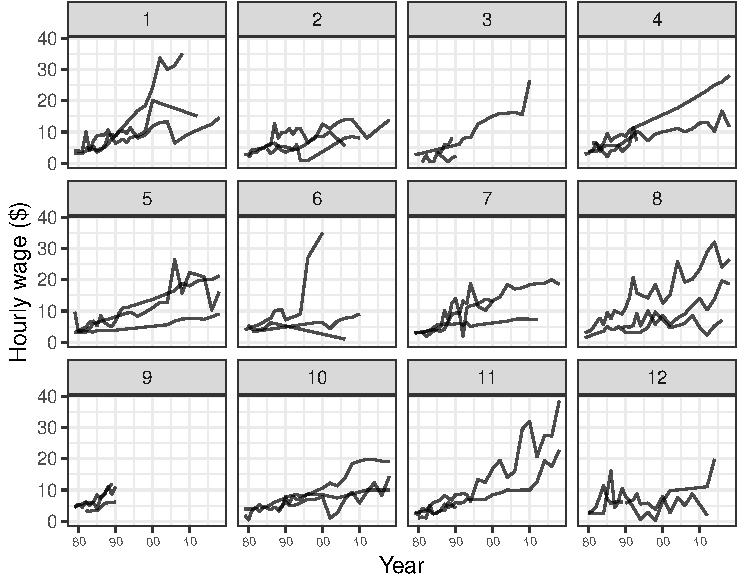
\includegraphics[width=1\linewidth]{figures/sample-plot-1} 

}

\caption{A glimpse of the refreshed data. Longitudinal profiles of wages from 1979-2018 are shown for a random sample of 36 individuals, divided into twelve subplots. Most individuals here experienced increasing wages over time, although there is considerable fluctuation from one year to another.}\label{fig:sample-plot}
\end{figure}

However, we can not be sure only by observing the summary statistics. Hence, we use visualisation techniques to investigate this matter. Figure \ref{fig:feature-plot} conveys a problem in the mean hourly wage values. Figure \ref{fig:feature-plot} A shows that some observations have an exceptionally high figure of wages, even more than US\$10,000 per hour. In Figure \ref{fig:feature-plot} B, we barely see any difference in the minimum, median, and maximum value of the wages since the distribution is heavily skewed to the right.

\begin{figure}

{\centering 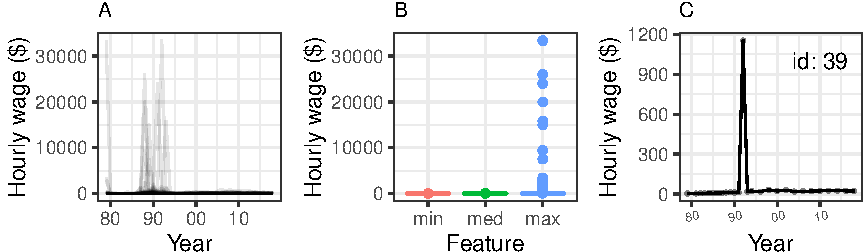
\includegraphics[width=432px]{figures/feature-plot-1} 

}

\caption{Summary plots to check the cleaned data reveal more cleaning is necessary: longitudinal profiles of wages for all individuals 1979-2018 (A), boxplots of minimum, median, and maximum wages of each individual (B), and one individual with an unusual wage relative to their years of data (C). Some values of hourly wages are unbelievable, and some individuals have extemely unusual wages in some years.}\label{fig:feature-plot}
\end{figure}

In Figure \ref{fig:high-wages}, we plot some respondents with a high value of mean hourly wages. We filter all of the IDs who earned more than US\$ 500 per hour on average. We find that these respondents only experienced one point of extremely high wages. Thus, we suspect that these high values are erroneous resulted from a data entry error.

Further, we take 36 samples randomly from the data and plot them, as shown in Figure \ref{fig:sample-plot}. It implies that not only that some observations earn extremely high figures of wages, but some also have reasonably fluctuated wages, for example, the IDs in panel numbers 5, 7, and 11. The plot also implies that the samples have a different pattern of mean hourly wages. Some have had flat wages for years but had a sudden increase in one particular year, then it gone down again, while the others experienced an upsurge in their wage, for instance, the IDs in panel 9.

The anomalies are also found in the total hours of work, where some observations work for 420 hours a week in total. According to Pergamit et al. (2001), one of the flaws of the NLSY79 employment data is that the NLSY79 collects the information of the working hours since the last interview. Thus, it might be challenging for the respondents to track the within-job hours' changes between survey years, especially for the respondents with fluctuated working hours or seasonal jobs. It even has been more challenging since 1994, where the respondents had to recall two years periods. This shortcoming might also contribute to the fluctuation of one's wages data.

\hypertarget{replacing-extreme-values}{%
\subsubsection{Replacing extreme values}\label{replacing-extreme-values}}

As part of the IDA, which is the model formulation, we build a robust linear regression model to treat the extreme values in the data. Robust linear regression yields an estimation robust to the influence of noise or contamination (Koller 2016). It also aims to detect the contamination by weighting each observation based on how ``well-behaved'' they are, known as robustness weight. Observations with lower robustness weight are suggested as an outlier by this method (Koller 2016).

Since we work with longitudinal data, we build the model for each ID instead of the overall data. The robust mixed model could be the best model to be employed in this case. However, this method is too computationally and memory expensive, especially for a large data set, like the NLSY79 data. Thus, the model for each ID is built utilizing the \texttt{nest} and \texttt{map} function from \texttt{tidyr} (Wickham 2020b) and \texttt{purrr} (Henry and Wickham 2020), respectively.

We build the model using the \texttt{rlm} function from \texttt{MASS} package (Venables and Ripley 2002). We set the \texttt{mean\_hourly\_wage} and \texttt{year} as the dependent and predictor, respectively. Furthermore, we use M-Estimation with Huber weighting, where the observation with a slight residual gets a weight of 1, while the larger the residual, the smaller the weight (less than 1) (UCLA: Statistical Consulting Group 2021). However, the challenging part of detecting the anomaly using the robustness weight is determining the weight threshold in which the observations are considered outliers. Moreover, it should be noted that not all the outliers are due to an error. Instead, it might be that one had reasonably increasing or decreasing wages in a particular period.

To minimize the risk of mistakenly identifying an outlier as an ``erroneous outlier,'' we simulate some thresholds and study how they affect the data. We find that 0.12 is the most reasonable value to be the threshold to minimize that drawback's risk because it still captures the sensible spikes in the data. In other words, we keep maintaining the natural variability of the wages while minimizing anomalies because of the error in the data recording. After deciding the threshold, we impute the observations whose weights are less than 0.12 with the models' predicted value. We then flag those observations in a new variable called \texttt{is\_pred}.

Figure \ref{fig:compare-plot} shows the mean hourly wage before and after the extreme values are replaced. It implies that the fluctuation can still be observed in the data after the treatment. However, the large spikes, which are considered ``erroneous outliers,'' are already eliminated from the data. Hence, the model produces a data set with a more reasonable degree of fluctuation.

\begin{figure}

{\centering 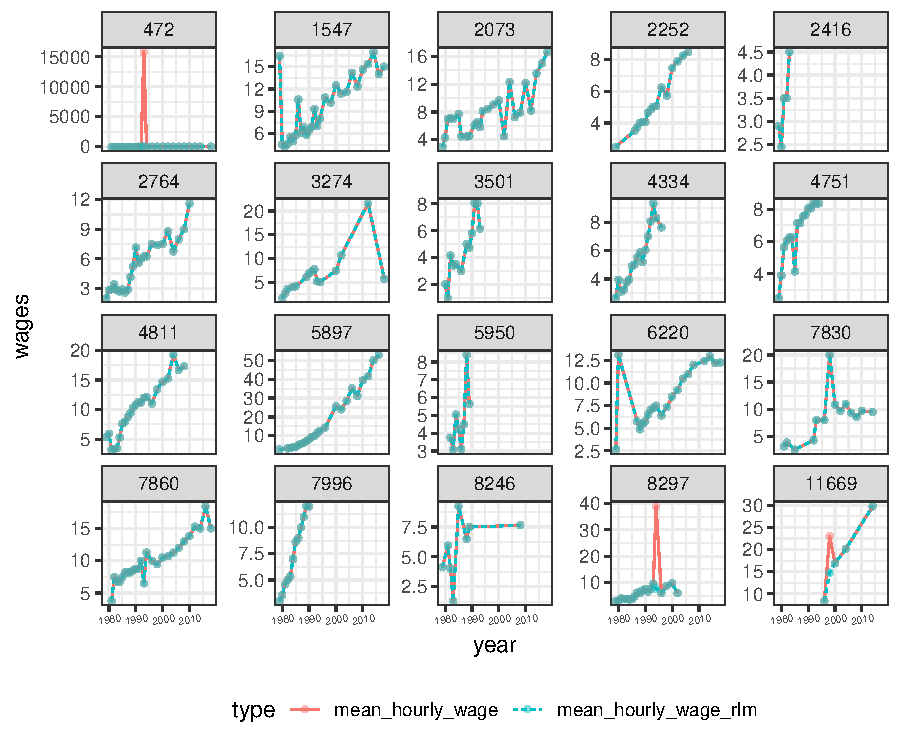
\includegraphics[width=432px]{figures/compare-plot-1} 

}

\caption{Comparison between the original and the treated mean hourly wage. The orange line portray the original value of mean hourly wage, while the turquoise line display the mean hourly wages value after the extreme values imputed with the robust linear model's prediction value. We can see that some extreme spikes has been reduced by the model.}\label{fig:compare-plot}
\end{figure}

Further, \ref{fig:comppict} A shows that after eliminating the extreme values, the highest value has decreased to be around \$350. The spikes are still observed but not as extreme as the original data set. In Figure \ref{fig:comppict} B), we plot the three features of mean hourly wages, namely the minimum, median, and maximum value, transformed to log scale. The plot implies that the skewness is slightly negative. We also see that the three features are overlapped each other. It indicates that some ID's minimum wages are higher than some ID's maximum wages.

\begin{figure}

{\centering 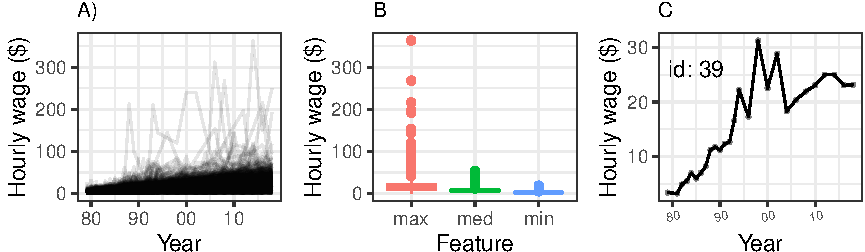
\includegraphics[width=432px]{figures/fixed-feature-plot-1} 

}

\caption{Re-make of the summary plots of the fully processed data suggest that the data is now in a reasonable state: longitudinal profiles of wages for all individuals 1979-2018 (A), boxplots of minimum, median, and maximum wages of each individual (B), and one individual with an unusual wage relative to their years of data (C). }\label{fig:fixed-feature-plot}
\end{figure}

Finally, we save the imputed data and set the appropriate data type for the variables. As our target data is the mean hourly wage of the high-school dropouts, we then subset the high-school graduate data set to have only the male-high school dropout data. We then make these three data sets and their processing documentation publicly available through an R data container package called \texttt{yowie}. The complete flow from the raw data to these data set is displayed in Figure \ref{fig:flow-chart}.

\begin{figure}

{\centering 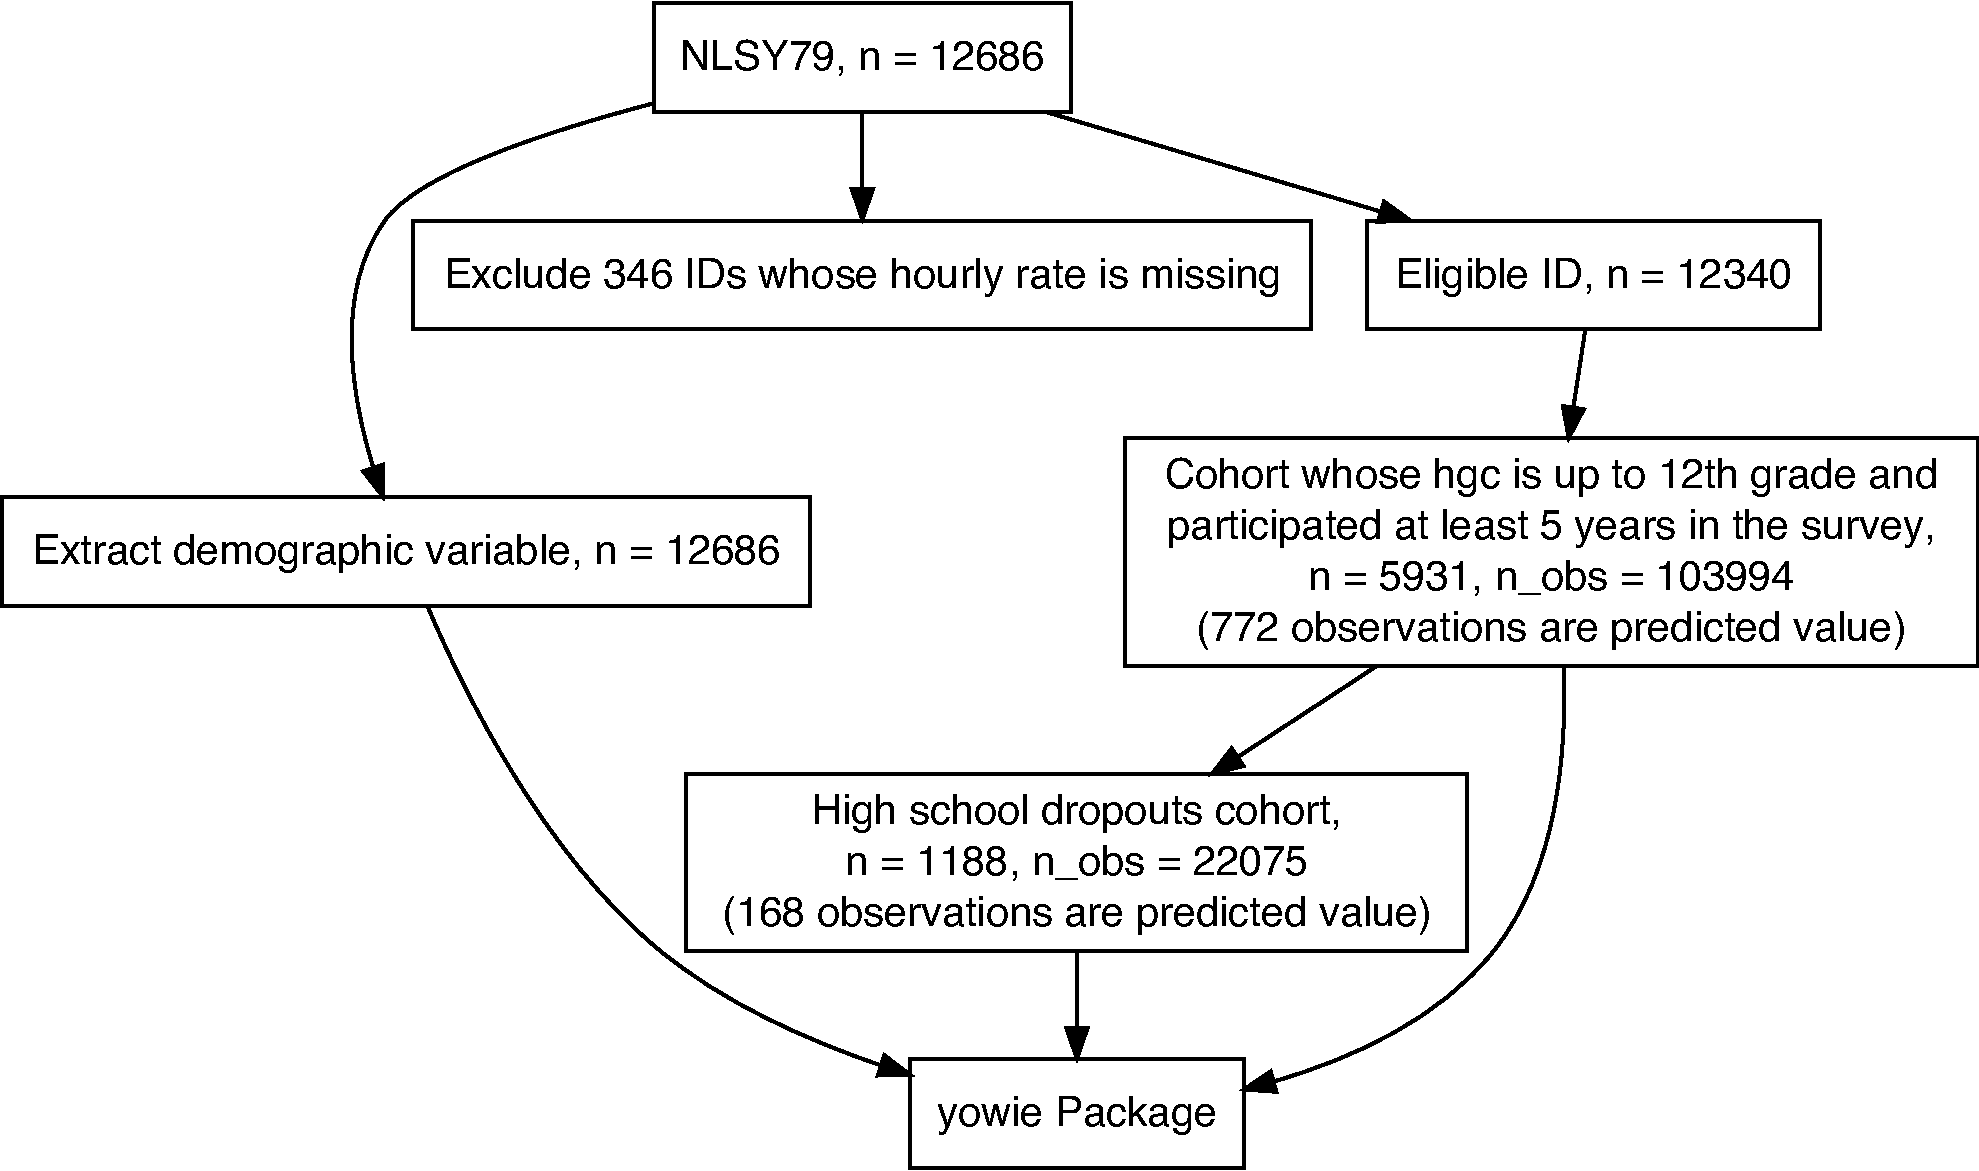
\includegraphics[width=468px]{figures/flow-chart-1} 

}

\caption{The stages of data filtering from the raw data to get three datasets contained yowie, n means the number of ID, while n\_obs means the number of observations.}\label{fig:flow-chart}
\end{figure}

\hypertarget{eda}{%
\section{Exploratory Data Analysis}\label{eda}}

This section will provide an example of how data sets could be used to do exploratory data analysis as in textbook data. We are interested in examining how the respondents experience changes in their wages based on their demographic characteristics. Thus, we use \texttt{wages} data instead of the refreshed \texttt{wages\_hs\_do} as it only has male respondents.

The statistics we use in measuring the change in wages experience is the slope of the wages of each respondent.
Using \texttt{key\_slope} function in \texttt{brolgar} (Tierney, Cook, and Prvan 2020), we perform linear regression with the log of mean hourly wage as the response variable and year as the predictor. Since we do modeling, it is important to look at the number of observations from each respondent. Figure \ref{fig:slope-nobs-plot} shows that the number of observations for each individual varies. Moreover, each number of observations seems to have an impact on the slope. Extreme values in slope are observed in a few observations, while the range of slope is more stable with more observations. Accordingly, we trim the data to only include respondents with at least 10 observations.

\begin{figure}

{\centering 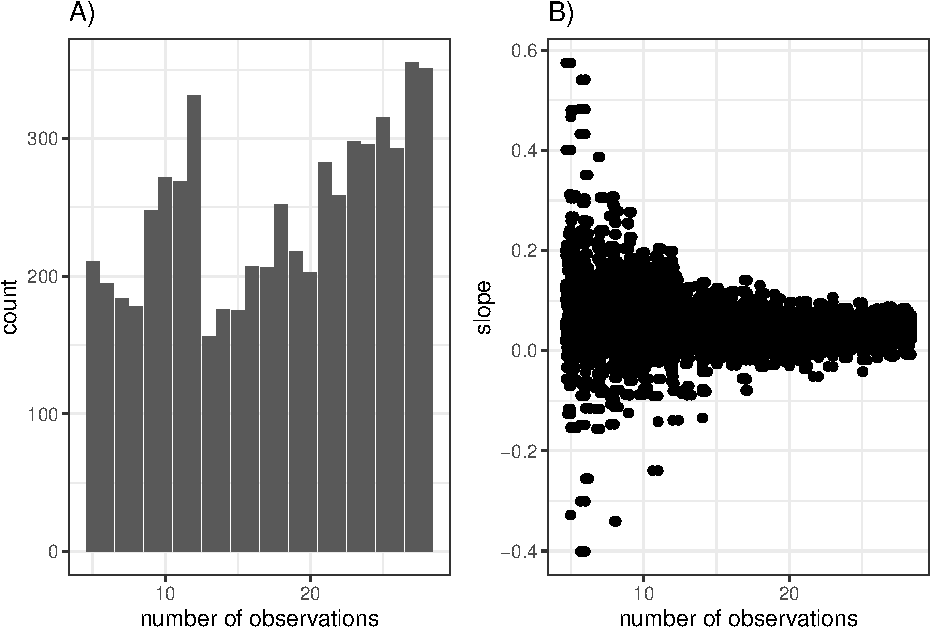
\includegraphics[width=468px]{figures/slope-nobs-plot-1} 

}

\caption{A) Distribution of observations. The numbers of rounds varies among respondents. Most of respondents participated in 28 rounds of survey. B) Distribution of wages slope by number of observations. The slopes' range are more stable with more observations.}\label{fig:slope-nobs-plot}
\end{figure}

We then create some visualizations of five respondents with the highest slope and five respondents with the lowest slope, henceforth referred to as top-5 slopes and bottom-5 slopes, respectively. We plot them based on their gender and education. Figure \ref{fig:slope-gender} shows top-5 slopes are dominated by males, while females dominate bottom-5 slopes. However, as this figure only shows a small portion of the data, we further inspect the gender wage gap.

\begin{figure}

{\centering 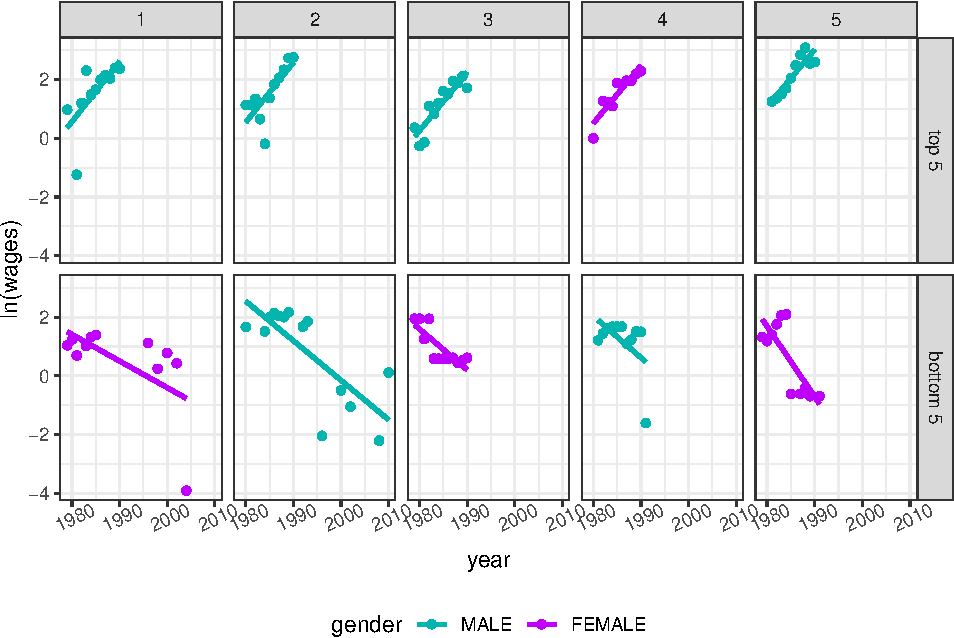
\includegraphics[width=468px]{figures/slope-gender-1} 

}

\caption{Wages slope over the years based on gender. Most of respondents who experienced high wages slope are males. In contrast, respondents who experienced lower wages slope are mostly females.}\label{fig:slope-gender}
\end{figure}

According to OECD (n.d.), the gender pay gap is the difference between the median wage of males and females relative to the median wage of males. We find that, as shown in \ref{fig:gap-gender}, over the years, females tend to earn fewer than males. For example, in 2018, females earned about 78 cents for every \$1 earned by males. The widest gender gaps were observed in the 1990s. However, as more males participated in the survey than females from year to year, these gaps could be affected by imbalance number of observations.

\begin{figure}

{\centering 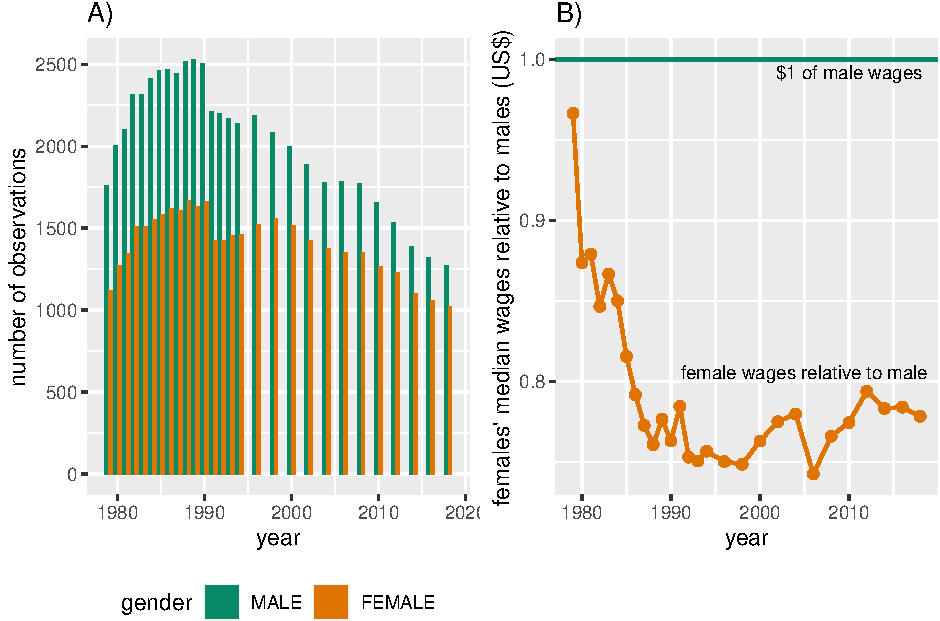
\includegraphics[width=0.9\linewidth]{figures/gap-gender-1} 

}

\caption{A) Number of observations by gender and by year. There are more males participated in survey than females. The number of observations decreased over the years. B) Gender wage gap or the median wages of females relatives to median wages of males. Females tend to earn fewer than males. For example, in 2018 females earn about 78 cents for every \$1 earned by males. Note that this is a crude measure as gap is calculated not based on other variable, such as experience and job class.}\label{fig:gap-gender}
\end{figure}

According to their highest education completed, both top-5 and bottom-5 slopes are dominated by people who completed high school. This is understandable since the respondents are mostly completed high school.

\begin{figure}

{\centering 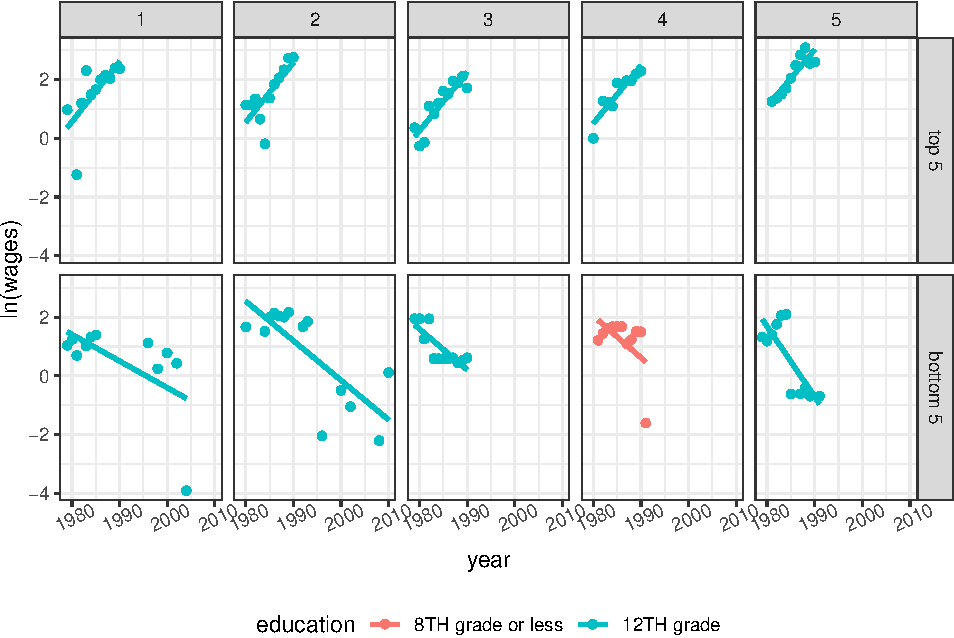
\includegraphics[width=468px]{figures/slope-educ-1} 

}

\caption{Wages slope over the years based on highest education completed. People who are in top-5 and bottom-5 wages are dominated by people who completed high school.}\label{fig:slope-educ}
\end{figure}

Further, we perform a linear regression to see the effect of education on wages experience.

\hypertarget{summary}{%
\section{Summary}\label{summary}}

This paper has performed stages to make open data suitable for textbook data or make it ready for research. In the first stage, we showed the steps performed to get the data from the NLSY79 database. Since the data format is untidy, we showed how the data had been tidied. After that, we conducted an initial data analysis to investigate and screen the quality of the data. We found and fixed the anomalous observations in the data set using the robust linear regression model with its predicted values. We also performed an example of exploratory data analysis using the cleaned data set.

This paper has also demonstrated data cleaning documentation by providing all of the codes in performing data tidying and initial data analysis. Thus, this paper provided an opportunity to continuously refresh the textbook data whenever the updated data is published in the NLSY79 database. It could be done by following the documentation of the code that is provided in this paper.

Moreover, the documentation also includes how we generated the robustness weight and how we decided the threshold of anomalous observations. It is also documented along with the flag of whether an observation is an imputed value or not. Accordingly, if somebody wishes to make another decision, it can be done by making a small change in the code provided. Further, this paper is also supplemented by a \texttt{shiny} (Chang et al. 2020) app as a simulation tool to customize the weight threshold.

Finally, this paper implies that data providers should design a database that is able to produce tidy data sets. A data provider should also check for data anomalies before the data publishing or at least provides a set of rules or threshold values. For example, in this case, is the threshold of reasonable wages. This will greatly support the data users to validate and set the same understanding of which data are considered outliers. Moreover, providing validation rules would facilitate any established data validation tool, such as \texttt{validate} (van der Loo and de Jonge 2021) package. In this case, we cannot use this handy validation package due to the absence of validation rules.

\hypertarget{acknowledgements}{%
\section{Acknowledgements}\label{acknowledgements}}

We would like to thank Aarathy Babu for the insight and discussion during the writing of this paper.

The entire analysis is conducted using \texttt{R} (R Core Team 2020) in \texttt{rstudio} using these packages: \texttt{tidyverse} (Wickham et al. 2019), \texttt{ggplot2} (Wickham 2016), \texttt{dplyr} (Wickham et al. 2020), \texttt{readr} (Wickham and Hester 2020), \texttt{tidyr} (Wickham 2020b), \texttt{stringr} (Wickham 2019), \texttt{purrr} (Henry and Wickham 2020), \texttt{broom} (Robinson, Hayes, and Couch 2021), \texttt{brolgar} (Tierney, Cook, and Prvan 2020), \texttt{patchwork} (Pedersen 2020), \texttt{kableExtra} (Zhu 2019), \texttt{MASS} (Venables and Ripley 2002), \texttt{janitor} (Firke 2020), \texttt{DiagrammeR} (Iannone 2020), \texttt{rsvg} (Ooms 2020), \texttt{webshot} (Chang 2019), \texttt{mgcv} (Wood 2003), \texttt{tsibble} (Wang, Cook, and Hyndman 2020), and \texttt{modelr} (Wickham 2020a). The paper are generated using \texttt{knitr} (Xie 2014), \texttt{rmarkdown} (Xie, Dervieux, and Riederer 2020), and \texttt{rticles} (Allaire et al. 2021).

\hypertarget{supplementary-materials}{%
\section{Supplementary Materials}\label{supplementary-materials}}

\begin{itemize}
\item
  \textbf{Codes} : R script to reproduce data tidying and cleaning are available in this \href{https://github.com/numbats/yowie/blob/master/data-raw/data_preprocessing.R}{Github Repository}.
\item
  \textbf{R Package \texttt{yowie}}:\texttt{yowie} is a data container R package that contains 3 datasets, namely the high school mean hourly wage data, high school dropouts mean hourly wage data, and demographic data of the NLSY79 cohort. This package could be accessed \href{https://github.com/numbats/yowie}{here}.
\item
  \textbf{shiny app}: An web interactive \texttt{shiny} app to run a simulation to customize the weight threshold. This app could be accessed \href{https://github.com/numbats/summer-wages-refresh/tree/main/app}{here}.
\end{itemize}

\hypertarget{references}{%
\section*{References}\label{references}}
\addcontentsline{toc}{section}{References}

\hypertarget{refs}{}
\begin{CSLReferences}{1}{0}
\leavevmode\hypertarget{ref-rticles}{}%
Allaire, JJ, Yihui Xie, R Foundation, Hadley Wickham, Journal of Statistical Software, Ramnath Vaidyanathan, Association for Computing Machinery, et al. 2021. \emph{Rticles: Article Formats for r Markdown}. \url{https://CRAN.R-project.org/package=rticles}.

\leavevmode\hypertarget{ref-webshot}{}%
Chang, Winston. 2019. \emph{Webshot: Take Screenshots of Web Pages}. \url{https://CRAN.R-project.org/package=webshot}.

\leavevmode\hypertarget{ref-shiny}{}%
Chang, Winston, Joe Cheng, JJ Allaire, Yihui Xie, and Jonathan McPherson. 2020. \emph{Shiny: Web Application Framework for r}. \url{https://CRAN.R-project.org/package=shiny}.

\leavevmode\hypertarget{ref-Chatfield1985TIEo}{}%
Chatfield, C. 1985. {``The Initial Examination of Data.''} \emph{Journal of the Royal Statistical Society. Series A. General} 148 (3): 214--53.

\leavevmode\hypertarget{ref-eliznlsy}{}%
Cooksey, Elizabeth C. 2017. {``Using the National Longitudinal Surveys of Youth (NLSY) to Conduct Life Course Analyses.''} In \emph{Handbook of Life Course Health Development}, edited by Richard M. Lerner Neal Halfon Christoper B. Forrest, 561--77. Cham: Springer. https://doi.org/\url{https://doi.org/10.1007/978-3-319-47143-3_23}.

\leavevmode\hypertarget{ref-DasuTamraparni2003Edma}{}%
Dasu, Tamraparni, and Theodore Johnson. 2003. \emph{Exploratory Data Mining and Data Cleaning}. Wiley Series in Probability and Statistics. Hoboken: WILEY.

\leavevmode\hypertarget{ref-janitor}{}%
Firke, Sam. 2020. \emph{Janitor: Simple Tools for Examining and Cleaning Dirty Data}. \url{https://CRAN.R-project.org/package=janitor}.

\leavevmode\hypertarget{ref-purrr}{}%
Henry, Lionel, and Hadley Wickham. 2020. \emph{Purrr: Functional Programming Tools}. \url{https://CRAN.R-project.org/package=purrr}.

\leavevmode\hypertarget{ref-HuebnerMariannePhD2016Asat}{}%
Huebner, Marianne, Werner Vach, and Saskia le Cessie. 2016. {``A Systematic Approach to Initial Data Analysis Is Good Research Practice.''} \emph{The Journal of Thoracic and Cardiovascular Surgery} 151 (1): 25--27.

\leavevmode\hypertarget{ref-HuebnerMarianne2020Haar}{}%
Huebner, Marianne, Werner Vach, Saskia le Cessie, Carsten Oliver Schmidt, and Lara Lusa. 2020. {``Hidden Analyses: A Review of Reporting Practice and Recommendations for More Transparent Reporting of Initial Data Analyses.''} \emph{BMC Medical Research Methodology} 20 (1): 61--61.

\leavevmode\hypertarget{ref-DiagrammeR}{}%
Iannone, Richard. 2020. \emph{DiagrammeR: Graph/Network Visualization}. \url{https://CRAN.R-project.org/package=DiagrammeR}.

\leavevmode\hypertarget{ref-KollerManuel2016rARP}{}%
Koller, Manuel. 2016. {``Robustlmm: An r Package for Robust Estimation of Linear Mixed-Effects Models.''} \emph{Journal of Statistical Software} 75 (6): 1--24.

\leavevmode\hypertarget{ref-OECD}{}%
OECD. n.d. {``Gender Wage Gap.''} https://data.oecd.org/earnwage/gender-wage-gap.htm.

\leavevmode\hypertarget{ref-rsvg}{}%
Ooms, Jeroen. 2020. \emph{Rsvg: Render SVG Images into PDF, PNG, PostScript, or Bitmap Arrays}. \url{https://CRAN.R-project.org/package=rsvg}.

\leavevmode\hypertarget{ref-opendata}{}%
Open Knowledge Foundation. 2021. {``Open Definition. Defining Open in Open Data, Open Content, and Open Knowledge.''} 2021. \url{http://opendefinition.org/od/2.1/en/}.

\leavevmode\hypertarget{ref-patchwork}{}%
Pedersen, Thomas Lin. 2020. \emph{Patchwork: The Composer of Plots}. \url{https://CRAN.R-project.org/package=patchwork}.

\leavevmode\hypertarget{ref-MichaelRPergamit2001DWTN}{}%
Pergamit, Michael R., Charles R. Pierret, Donna S. Rothstein, and Jonathan R. Veum. 2001. {``Data Watch: The National Longitudinal Surveys.''} \emph{The Journal of Economic Perspectives} 15 (2): 239--53.

\leavevmode\hypertarget{ref-R}{}%
R Core Team. 2020. \emph{R: A Language and Environment for Statistical Computing}. Vienna, Austria: R Foundation for Statistical Computing. \url{https://www.R-project.org/}.

\leavevmode\hypertarget{ref-broom}{}%
Robinson, David, Alex Hayes, and Simon Couch. 2021. \emph{Broom: Convert Statistical Objects into Tidy Tibbles}. \url{https://CRAN.R-project.org/package=broom}.

\leavevmode\hypertarget{ref-SingerJudithD2003Alda}{}%
Singer, Judith D, and John B Willett. 2003. \emph{Applied Longitudinal Data Analysis: Modeling Change and Event Occurrence}. Oxford u.a: Oxford Univ. Pr.

\leavevmode\hypertarget{ref-nlsy79}{}%
The U.S. Bureau of Labor Statistics. n.d. {``National Longitudinal Survey of Youth 1979.''} Available at \url{https://www.nlsinfo.org/content/cohorts/nlsy79} (2021/25/02).

\leavevmode\hypertarget{ref-brolgar}{}%
Tierney, Nicholas, Di Cook, and Tania Prvan. 2020. \emph{Brolgar: BRowse over Longitudinal Data Graphically and Analytically in r}. \url{https://github.com/njtierney/brolgar}.

\leavevmode\hypertarget{ref-tukey}{}%
Tukey, John W. (John Wilder). 1977. \emph{Exploratory Data Analysis}. Addison-Wesley Series in Behavioral Science. Reading, Mass.: Addison-Wesley Pub. Co.

\leavevmode\hypertarget{ref-rlm}{}%
UCLA: Statistical Consulting Group. 2021. {``Robust Regression \textbar{} r Data Analysis Examples.''} February 2021. \url{https://stats.idre.ucla.edu/r/dae/robust-regression/}.

\leavevmode\hypertarget{ref-validate}{}%
van der Loo, Mark P. J., and Edwin de Jonge. 2021. {``Data Validation Infrastructure for {R}.''} \emph{Journal of Statistical Software} 97 (10): 1--31. \url{https://doi.org/10.18637/jss.v097.i10}.

\leavevmode\hypertarget{ref-mass}{}%
Venables, W. N., and B. D. Ripley. 2002. \emph{Modern Applied Statistics with s}. Fourth. New York: Springer. \url{http://www.stats.ox.ac.uk/pub/MASS4}.

\leavevmode\hypertarget{ref-tsibble}{}%
Wang, Earo, Dianne Cook, and Rob J Hyndman. 2020. {``A New Tidy Data Structure to Support Exploration and Modeling of Temporal Data.''} \emph{Journal of Computational and Graphical Statistics} 29 (3): 466--78. \url{https://doi.org/10.1080/10618600.2019.1695624}.

\leavevmode\hypertarget{ref-WickhamHadley2014TD}{}%
Wickham, Hadley. 2014. {``Tidy Data.''} \emph{Journal of Statistical Software} 59 (10): 1--23.

\leavevmode\hypertarget{ref-ggplot2}{}%
---------. 2016. \emph{Ggplot2: Elegant Graphics for Data Analysis}. Springer-Verlag New York. \url{https://ggplot2.tidyverse.org}.

\leavevmode\hypertarget{ref-stringr}{}%
---------. 2019. \emph{Stringr: Simple, Consistent Wrappers for Common String Operations}. \url{https://CRAN.R-project.org/package=stringr}.

\leavevmode\hypertarget{ref-modelr}{}%
---------. 2020a. \emph{Modelr: Modelling Functions That Work with the Pipe}. \url{https://CRAN.R-project.org/package=modelr}.

\leavevmode\hypertarget{ref-tidyr}{}%
---------. 2020b. \emph{Tidyr: Tidy Messy Data}. \url{https://CRAN.R-project.org/package=tidyr}.

\leavevmode\hypertarget{ref-tidyverse}{}%
Wickham, Hadley, Mara Averick, Jennifer Bryan, Winston Chang, Lucy D'Agostino McGowan, Romain François, Garrett Grolemund, et al. 2019. {``Welcome to the {tidyverse}.''} \emph{Journal of Open Source Software} 4 (43): 1686. \url{https://doi.org/10.21105/joss.01686}.

\leavevmode\hypertarget{ref-dplyr}{}%
Wickham, Hadley, Romain François, Lionel Henry, and Kirill Müller. 2020. \emph{Dplyr: A Grammar of Data Manipulation}. \url{https://CRAN.R-project.org/package=dplyr}.

\leavevmode\hypertarget{ref-readr}{}%
Wickham, Hadley, and Jim Hester. 2020. \emph{Readr: Read Rectangular Text Data}. \url{https://CRAN.R-project.org/package=readr}.

\leavevmode\hypertarget{ref-mgcv}{}%
Wood, S. N. 2003. {``Thin-Plate Regression Splines.''} \emph{Journal of the Royal Statistical Society (B)} 65 (1): 95--114.

\leavevmode\hypertarget{ref-knitr}{}%
Xie, Yihui. 2014. {``Knitr: A Comprehensive Tool for Reproducible Research in {R}.''} In \emph{Implementing Reproducible Computational Research}, edited by Victoria Stodden, Friedrich Leisch, and Roger D. Peng. Chapman; Hall/CRC. \url{http://www.crcpress.com/product/isbn/9781466561595}.

\leavevmode\hypertarget{ref-rmarkdown}{}%
Xie, Yihui, Christophe Dervieux, and Emily Riederer. 2020. \emph{R Markdown Cookbook}. Boca Raton, Florida: Chapman; Hall/CRC. \url{https://bookdown.org/yihui/rmarkdown-cookbook}.

\leavevmode\hypertarget{ref-kableExtra}{}%
Zhu, Hao. 2019. \emph{kableExtra: Construct Complex Table with 'Kable' and Pipe Syntax}. \url{https://CRAN.R-project.org/package=kableExtra}.

\end{CSLReferences}


\bibliographystyle{Chicago}

\end{document}
